\section{Results}
\label{sec:results}
\subsection{Models}
The results of this measurement for the \cconepi and \ccpi
channels are presented in the following figures.  They are compared
with calculations from the theoretical work of Athar, Chaukin, and
Singh (ACS)~\cite{Athar} and the event generators GENIE~\cite{Andreopoulos201087}, NEUT~\cite{Hayato:2009zz}, 
and NuWro~\cite{Golan:2012wx}.  Predictions from the GiBUU model can be found in Refs.~\cite{gibuu-minerva, gibuu_mnv}.  Each prediction includes
models for the initial neutrino interaction, the nuclear structure
affecting the initial interaction, and
the FSI of the particles produced.  For resonance production, GENIE and NEUT use
the model of Rein and Sehgal~\cite{Rein:1980wg} without including resonance interference and with varying 
treatments of nuclear structure.  NuWro includes only the $\Delta$(1232) resonance, using the Adler model~\cite{nuwro_res,nuwro_res2}, 
and ACS uses the parameterization of Schreiner and Von Hippel~\cite{acs_res} and contains medium 
modifications to the $\Delta$ mass and decay width.  

\begingroup
\squeezetable
\begin{table*}[ht]
\begin{tabular}{l|l|l|l|l|l}
\hline\hline
Model & Nucleon Resonance & Nonresonance & Nucleon Momentum & $\Delta$ Modifications & FSI \\ 
\hline 
ACS~\cite{Athar} & Schreiner--Von Hippel~\cite{acs_res} & None & local relativistic & $\Delta$ mass and & attenuation only~\cite{VicenteVacas:1994} \\ 
    & & & Fermi gas & decay width & \\
\hline
GENIE~\cite{Andreopoulos201087} 2.6.2 & Rein--Sehgal~\cite{Rein:1980wg} & Bodek--Yang~\cite{Bodek:2004pc} with & global relativistic & no & effective cascade \\
    & without interference & extrapolation to lower $W$ & Fermi gas & & \\
\hline
NEUT~\cite{Hayato:2009zz} 5.3.3 & Rein--Sehgal & Rein--Sehgal & global relativistic & yes, via FSI model & Salcedo--Oset~\cite{Salcedo:1987md}, \\
    & without interference & & Fermi gas & & full cascade \\
\hline
NuWro~\cite{Golan:2012wx} & Adler~\cite{nuwro_res,nuwro_res2}, & Bodek--Yang with & global relativistic & yes, via FSI model & Salcedo--Oset, \\
    & $\Delta$(1232) only & extrapolation to lower $W$ & Fermi gas & & full cascade \\

\hline\hline
\end{tabular}
\caption{Summary of the models presented in this paper.}
\label{tab:models}
\end{table*}
\endgroup

NEUT takes the nonresonant interaction from Rein and Sehgal; ACS has no nonresonant mechanisms; 
GENIE and NuWro have similar approaches, using the model of 
Bodek and Yang~\cite{Bodek:2004pc} above the resonance region
and smoothly extrapolating it to lower $W$ to converge with 
the resonance model.  All models must choose between matching
the ANL~\cite{Radecky:1981fn} and BNL~\cite{Kitagaki:1986ct} data 
for charged-current pion production from 
nucleon targets because the BNL data is about 40\% larger than the 
ANL data for neutrino energies of $\sim$2 GeV.  While the
GENIE fit is midway between the two data sets, NEUT and NuWro fits
are closer to the ANL result.  

GENIE, NEUT, and NuWro use
a relativistic Fermi gas model for the nucleon momentum distribution, while
ACS uses a local Fermi gas model in which the Fermi momentum depends
on the radial distance from the center of the nucleus.  For FSI, NEUT and 
NuWro use the Salcedo--Oset model~\cite{Salcedo:1987md} in a cascade 
formalism which has nuclear medium corrections, while GENIE uses an effective cascade 
model which has similar agreement with pion-nucleus data.  ACS uses a model which includes 
pion attenuation, but not inelastic scattering which changes the pion 
energy and angle~\cite{VicenteVacas:1994}.  Thus, a calculation with 
excellent nuclear medium effects but incomplete FSI (ACS) is compared with 
calculations with simple nuclear structure and detailed FSI (GENIE, NuWro, NEUT).  
Table~\ref{tab:models} summarizes the models used by the predictions shown in this paper.


\subsection{\cconepi\ results}
The measured $d\sigma/d\theta_\pi$ for the \cconepi analysis
is shown in Fig.~\ref{fig:piangle-1pi}, along with predictions 
from the models discussed above.  The $\chi^2$ between the data and 
model predictions are listed in Table~\ref{tab:chi2}.  
The effect of FSI, shown in the comparison between 
the GENIE ``hA FSI'' and ``no FSI'' curves, is to deplete (increase) 
the forward (backward) angle cross section.  Both the absolute and 
shape measurements show a clear preference for models that implement FSI with a full or effective cascade model.  
In particular, the ``no FSI'' and ACS predictions do not 
describe the relative cross section for forward- and backward-going pions.

\begin{figure}[h]
\centering
\subfloat[] {
    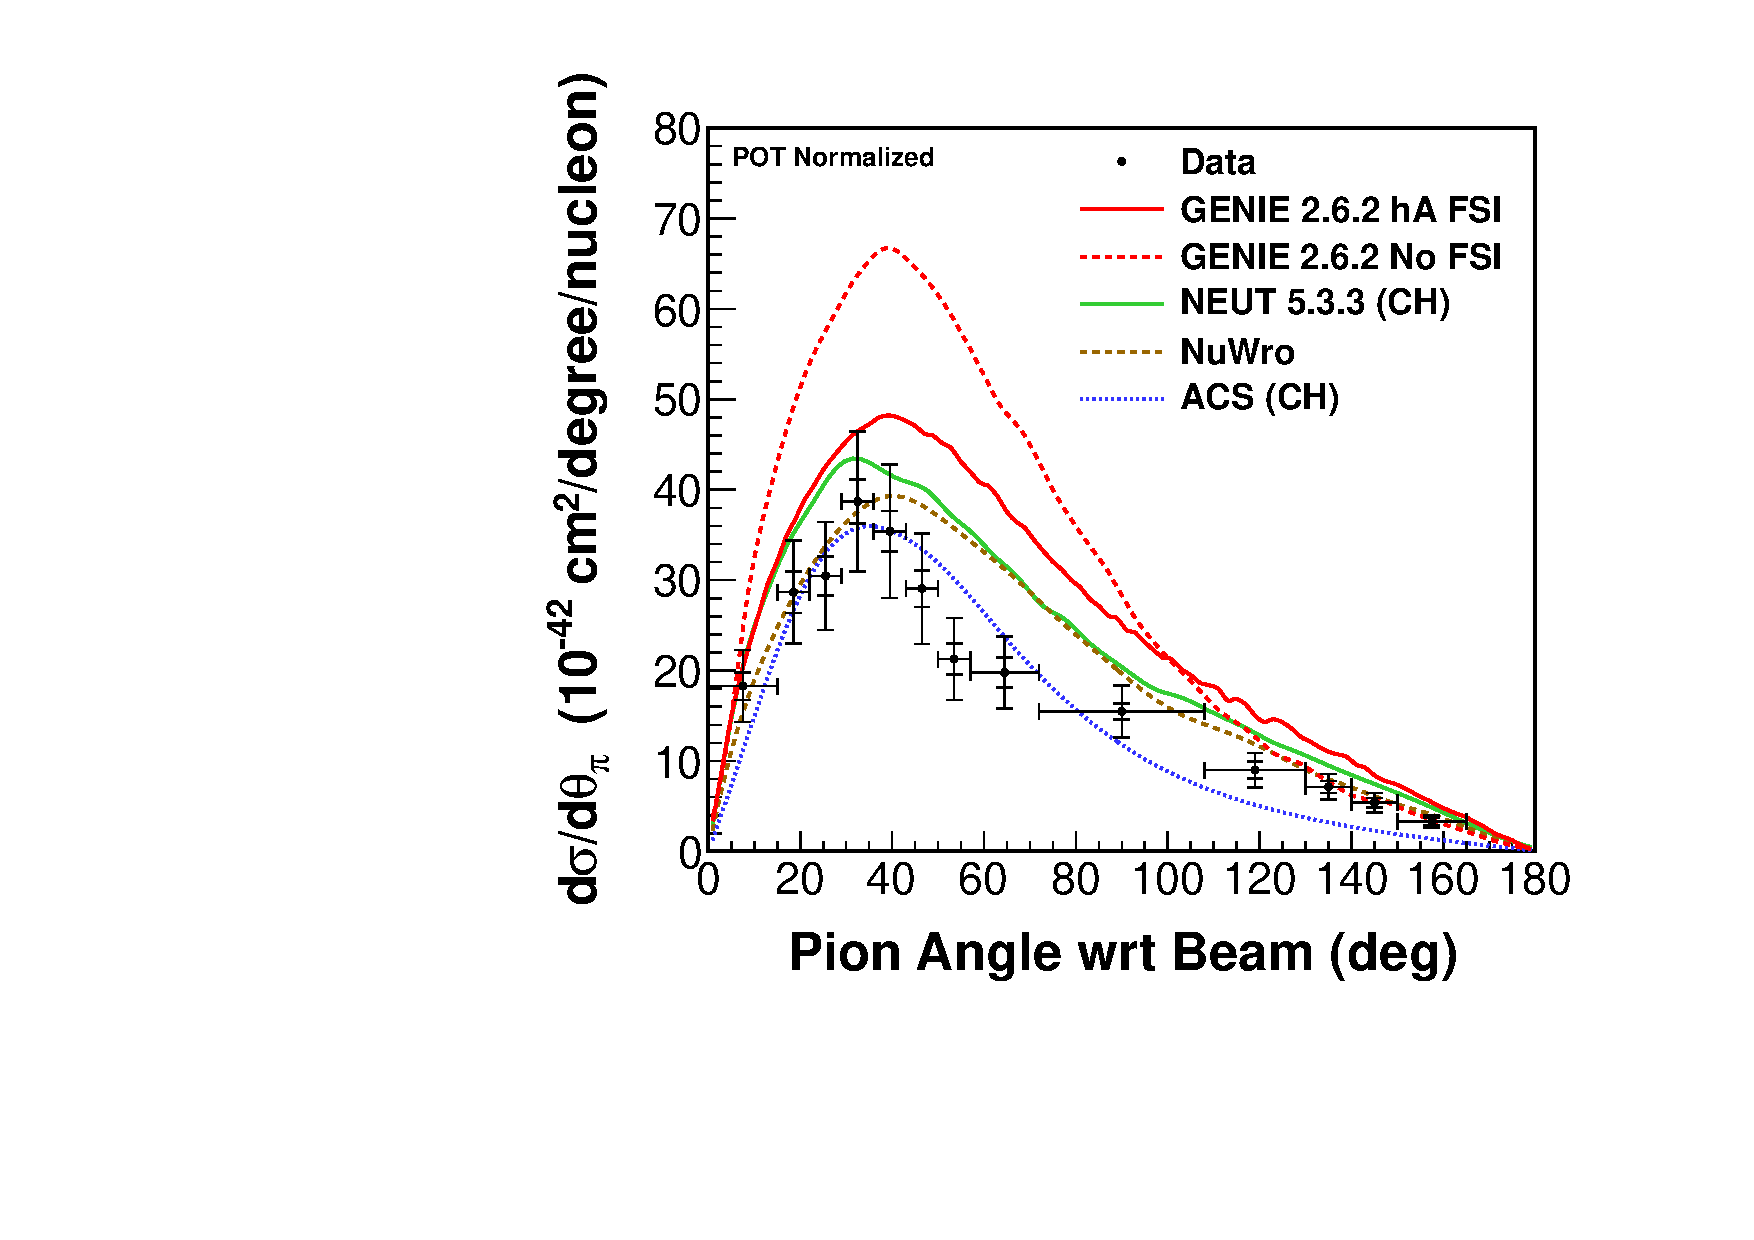
\includegraphics[width=\columnwidth]{figures/modelComp_POT_pi_theta}
}
\qquad
\subfloat[] {
    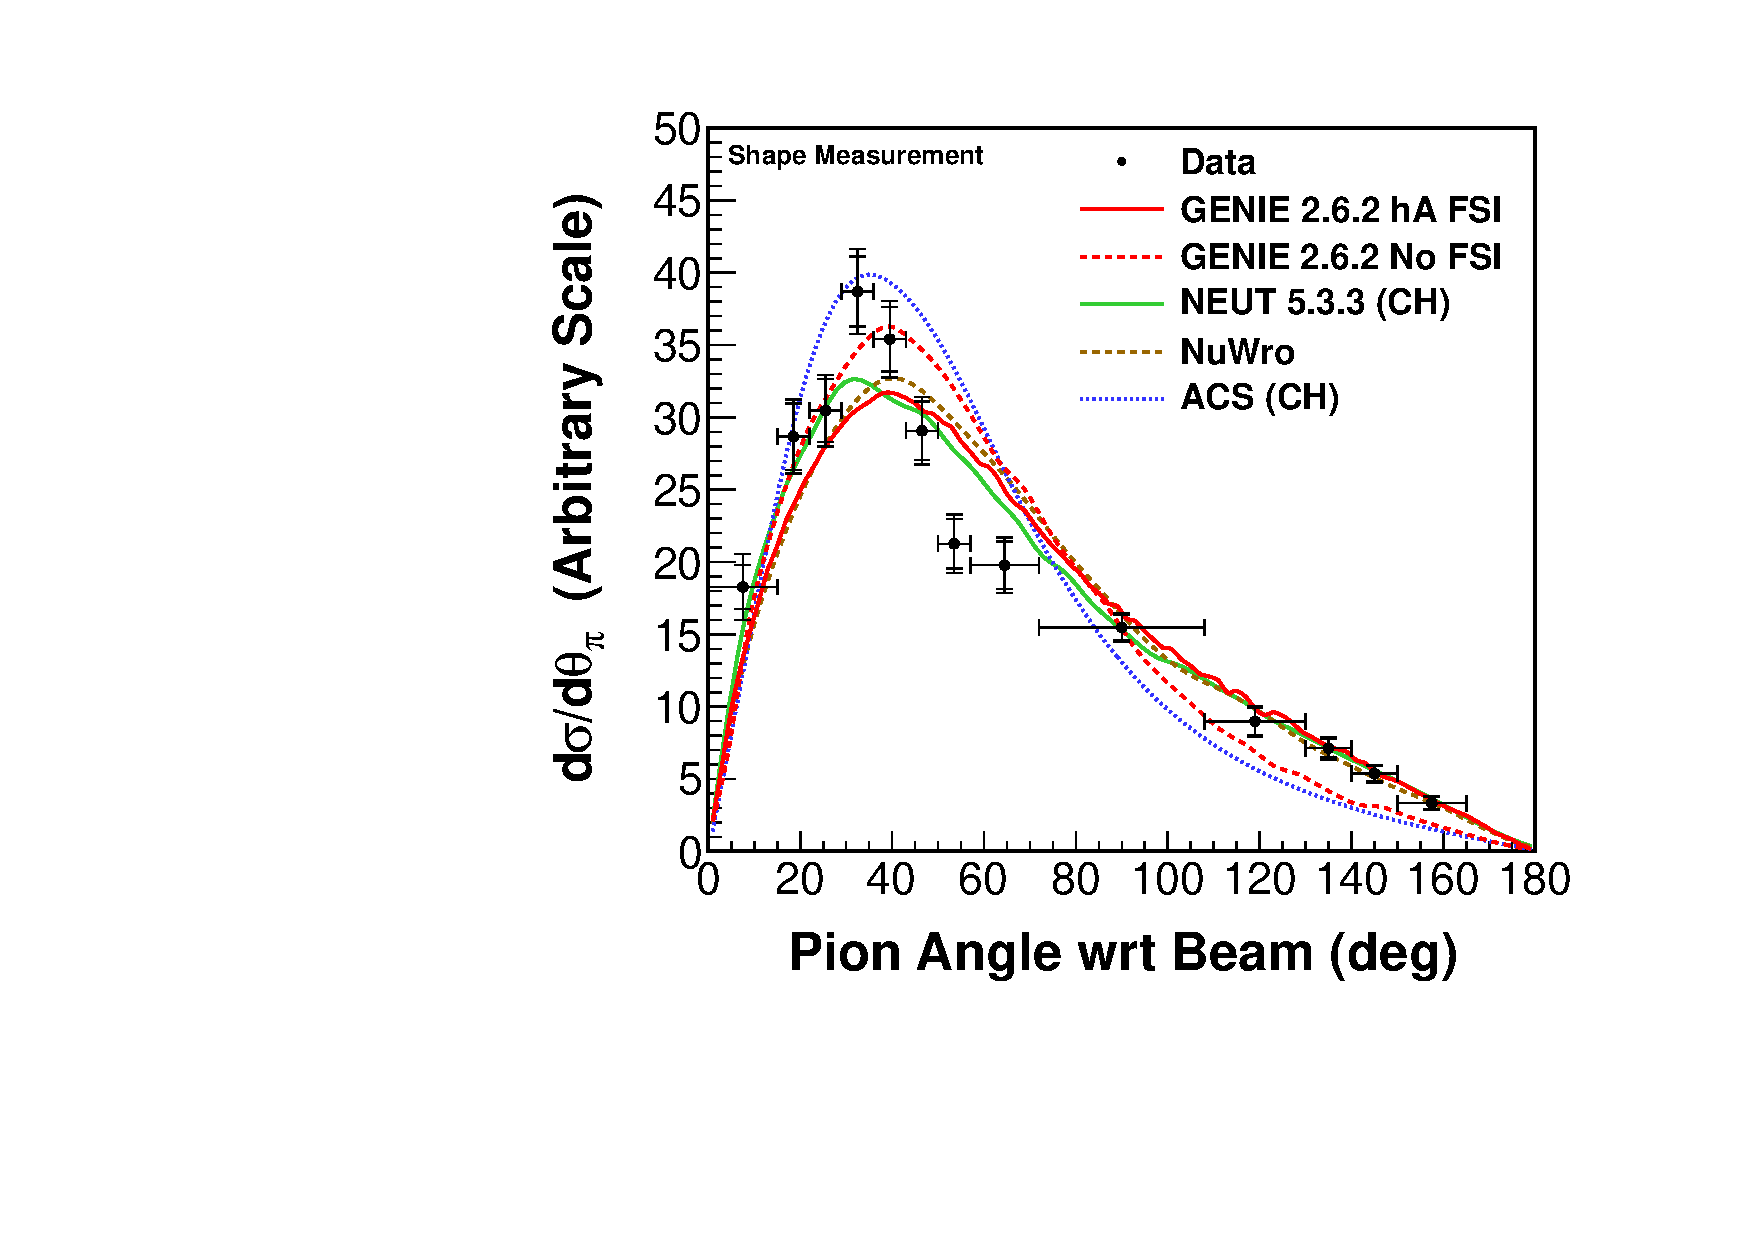
\includegraphics[width=\columnwidth]{figures/modelComp_AN_pi_theta}
}
%    \vspace{-7pt}
\caption{\cconepi $d\sigma / d\theta_\pi$ (top) and its shape (bottom) compared to the GENIE, ACS, NEUT, and NuWro models.
The shape predictions are normalized to the integral of the data.  The inner (outer) error bars correspond to the statistical (total) uncertainties.}
%    \vspace{-10pt}
\label{fig:piangle-1pi}
\end{figure}

\begingroup
\squeezetable
\begin{table}[h]
\begin{tabular}{l|cc}
\hline\hline
Model & Absolute $\chi^{2}$ & Shape $\chi^{2}$ \\ 
\hline 
ACS (CH) & 78 & 89 \\ 
GENIE 2.6.2 hA FSI & 104 & 41 \\
GENIE 2.6.2 No FSI & 234 & 72 \\
NEUT 5.3.3 (CH) & 50 & 26 \\
NuWro & 67 & 46 \\
\hline\hline
ACS (CH) & 40 & 34  \\ 
GENIE 2.6.2 hA FSI & 21 & 7.4 \\
GENIE 2.6.2 No FSI & 105 & 23 \\
NEUT 5.3.3 (CH) & 26 & 13 \\
NuWro & 25 & 16 \\
\hline\hline
\end{tabular}
\caption{Top: Absolute (shape) $\chi^{2}$ with 13 (12) degrees of freedom between the \cconepi $d\sigma / d\theta_\pi$ measurement and various models. 
Bottom: Corresponding \cconepi $d\sigma / dT_\pi$ $\chi^{2}$ with 7 (6) degrees of freedom.}
\label{tab:chi2}
\end{table}
\endgroup
 
The shape of $d\sigma/d\theta_\pi$ could be 
sensitive to the $\Delta \rightarrow \pi$ decay angle distribution.  
GENIE and NuWro use an isotropic decay 
distribution while NEUT assumes the anisotropy in the original Rein-Sehgal 
model~\cite{Rein:1980wg}.  ACS calculates specific anisotropies 
for the $\Delta^{++}$ and the $\Delta^+$ separately.  
The larger effect, however, is the implementation of FSI.  

The measured \cconepi $d\sigma/dT_\pi$ is shown in  
Fig.~\ref{fig:pike-1pi} along with the model predictions.  The $\chi^2$ 
calculations are provided in Table~\ref{tab:chi2}.
FSI suppresses the charged pion production cross section through pion 
absorption and charge exchange, and migrates pions to lower energies 
through scattering.  These interactions are highly energy dependent, 
peaking between 100 and 220~MeV~\cite{Leitner:2008wx}, and significantly 
modify the shape of $d\sigma/dT_\pi$.  The significant reduction in the total cross section is seen
by comparing the solid and dashed GENIE predictions in the absolute measurement, while the energy dependence 
of the FSI can be clearly seen by comparing the GENIE predictions for the shape measurement.  
The data are in best agreement with models that implement full or effective particle cascade FSI algorithms.     

\begin{figure}[ht]
\centering
\subfloat[] {
    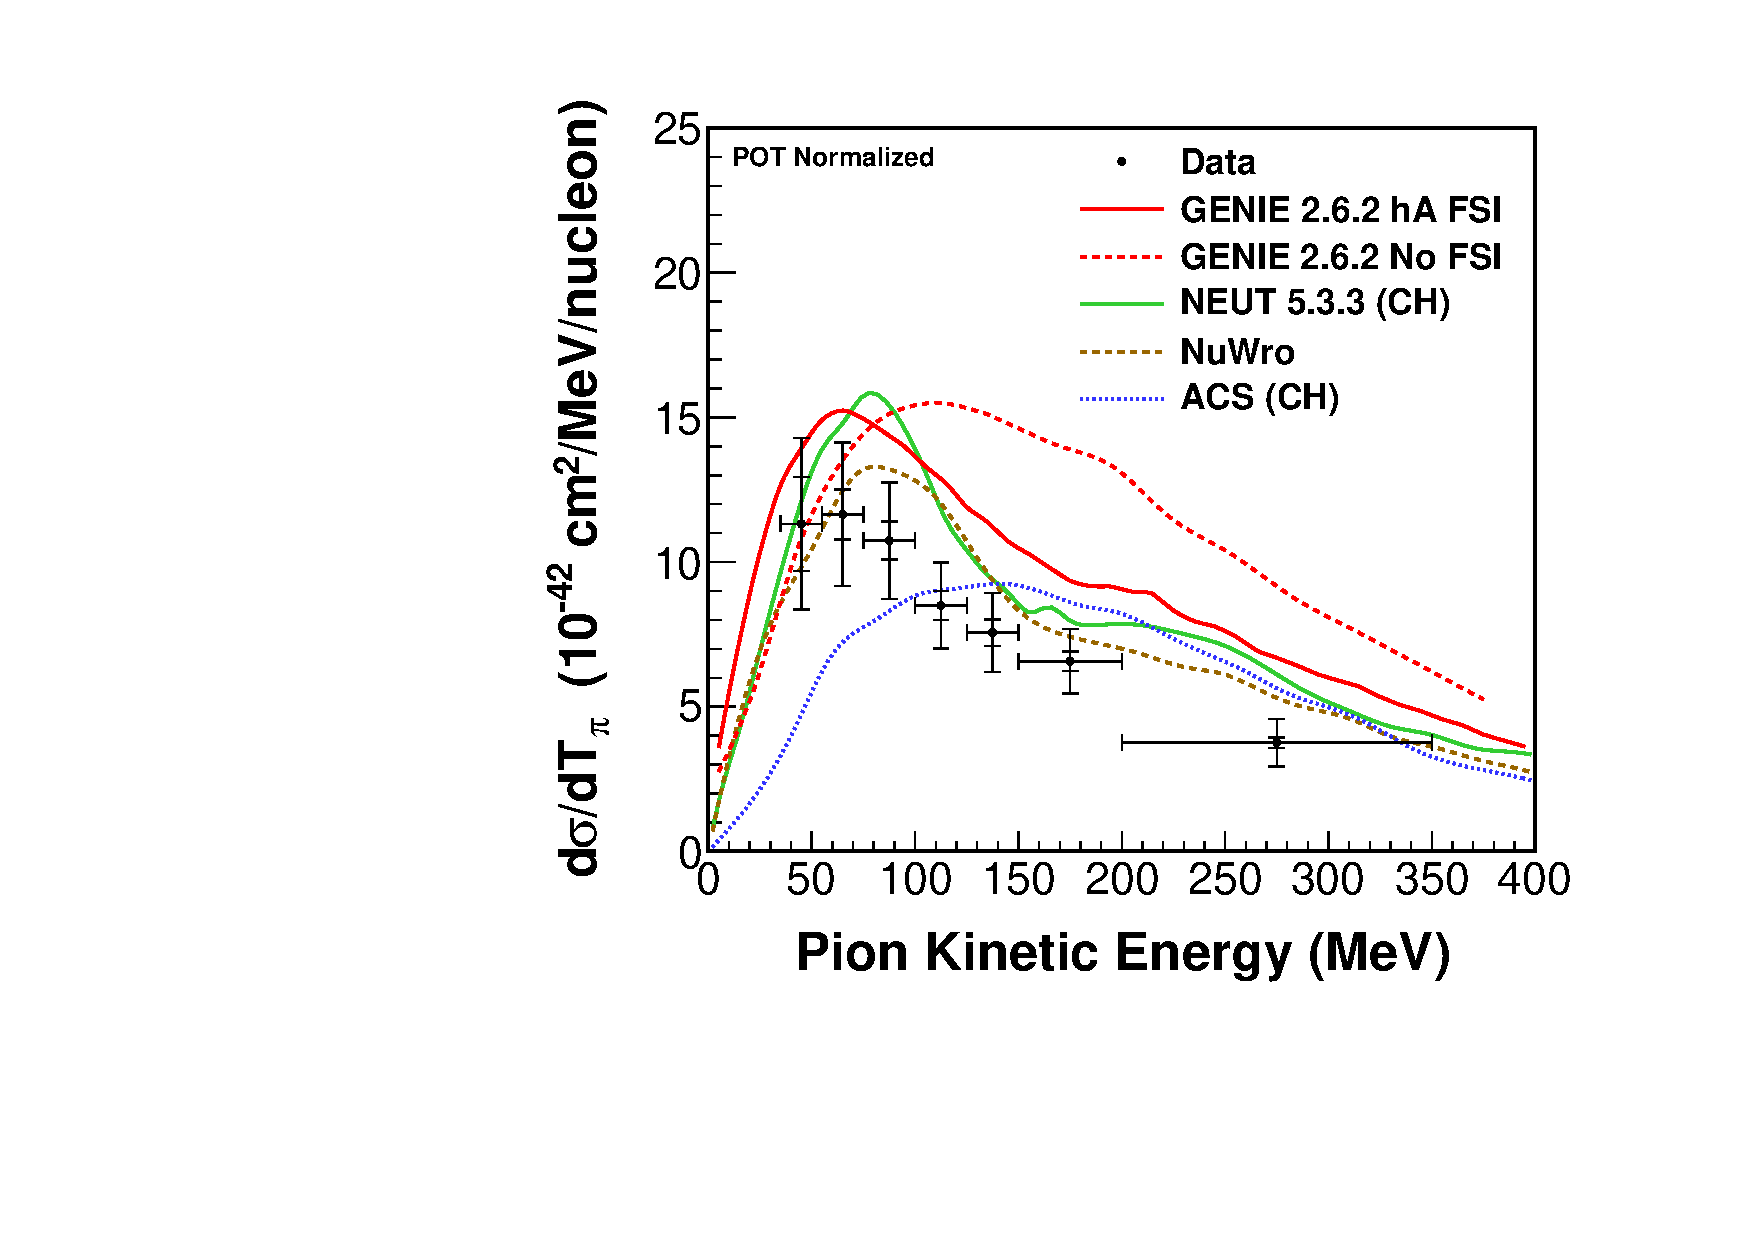
\includegraphics[width=\columnwidth]{figures/modelComp_POT_pi_ke}
}
\qquad
\subfloat[] {
    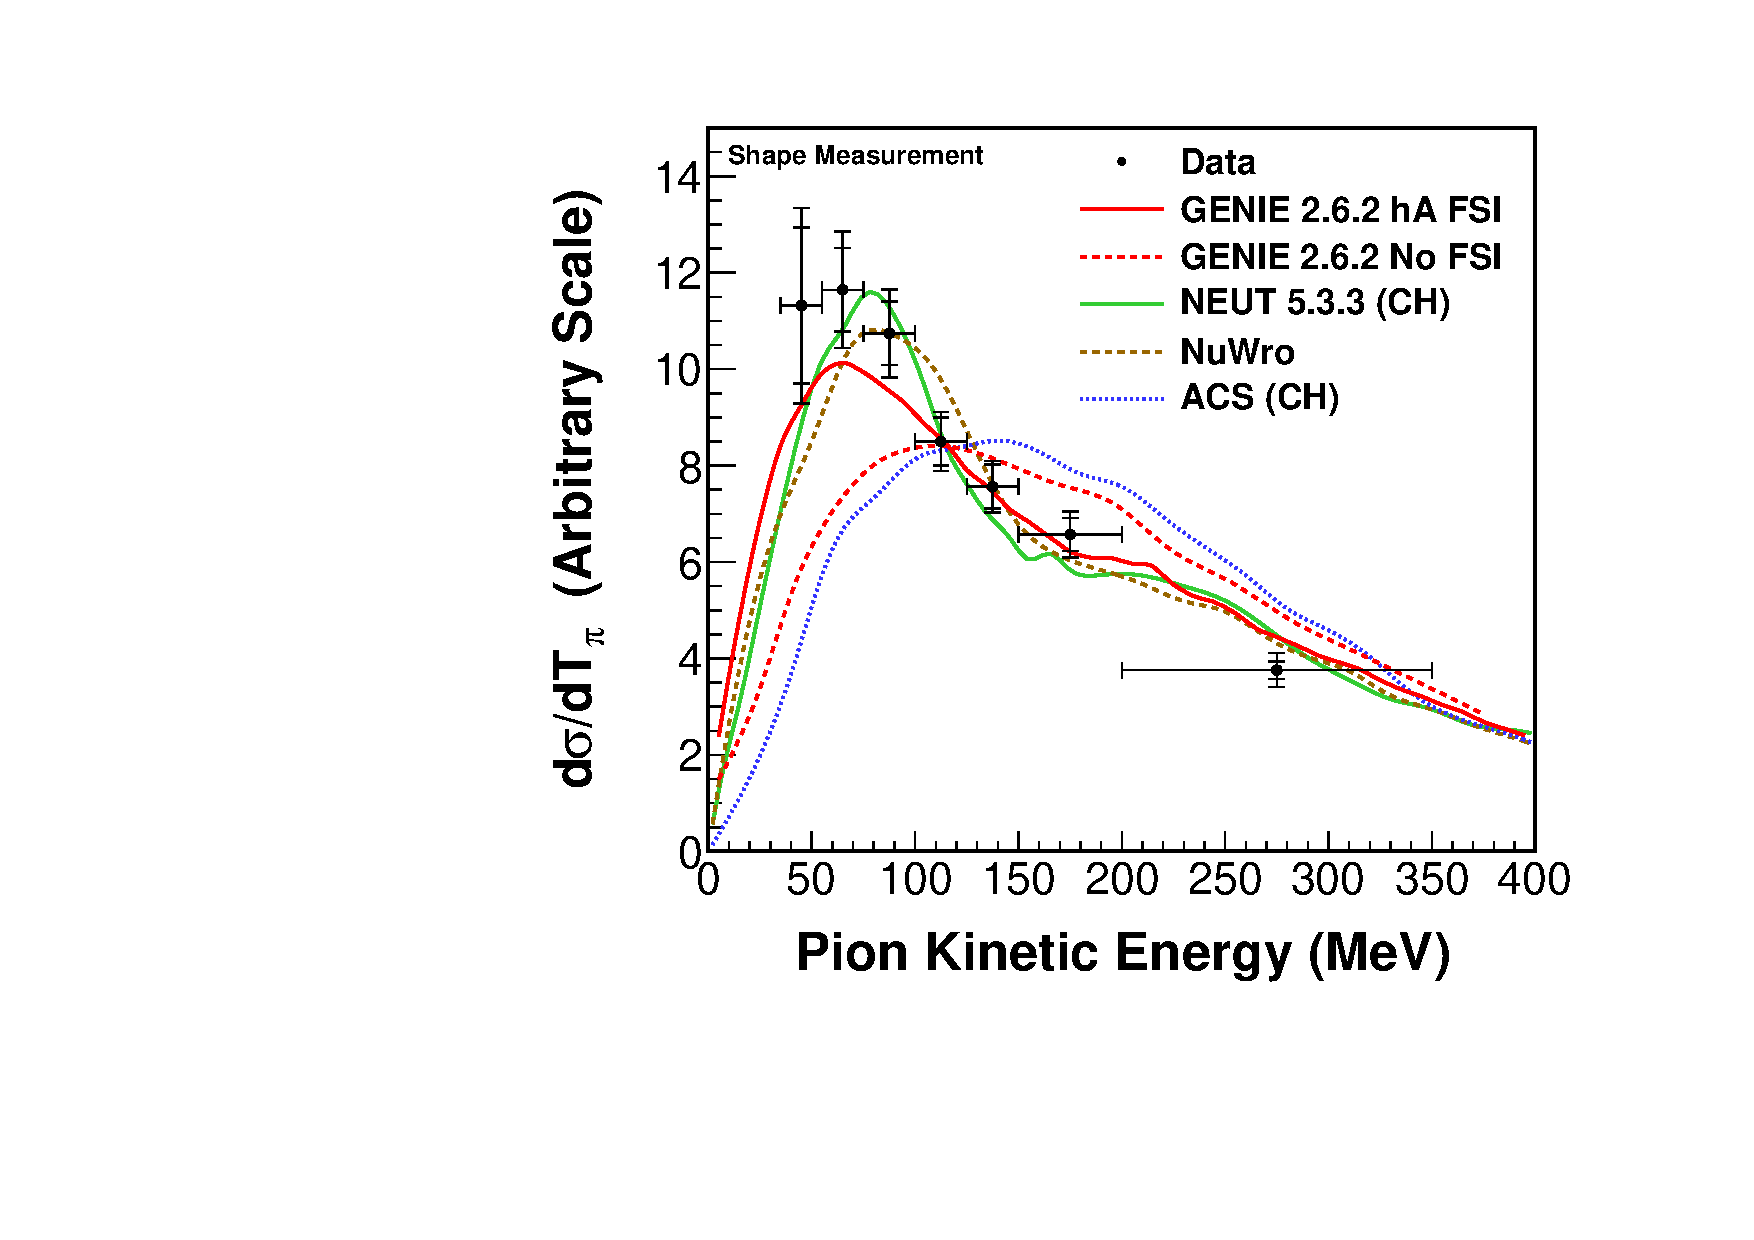
\includegraphics[width=\columnwidth]{figures/modelComp_AN_pi_ke}
}
%    \vspace{-7pt}
\caption{\cconepi $d\sigma / d\Tpi$ (top) and its shape (bottom) compared to the GENIE, ACS, NEUT, and NuWro models.
The shape predictions are normalized to the integral of the data.  The inner (outer) error bars correspond to the statistical (total) uncertainties.}
%    \vspace{-10pt}
\label{fig:pike-1pi}
\end{figure}

The shape of $d\sigma/d\Tpi$ is compared with the GENIE calculation subdivided by 
FSI channel in Fig.~\ref{fig:pike-1pi-AN-FSI}.  Effects of pion
absorption are significant but not directly seen because those
pions cannot be in the final state.  Inelastic scattering 
is the dominant contributor because the interaction probability is large
and the energy is significantly reduced.  Elastic scattering is also 
significant but does not affect the energy spectrum.  The calculation 
would agree with the data shape better if the inelastic
scattering contribution were increased within the estimated error
in the total pion inelastic cross section data ($\pm$40\%~\cite{Ashery:1981tq}).  

\begin{figure}[tp]
\centering
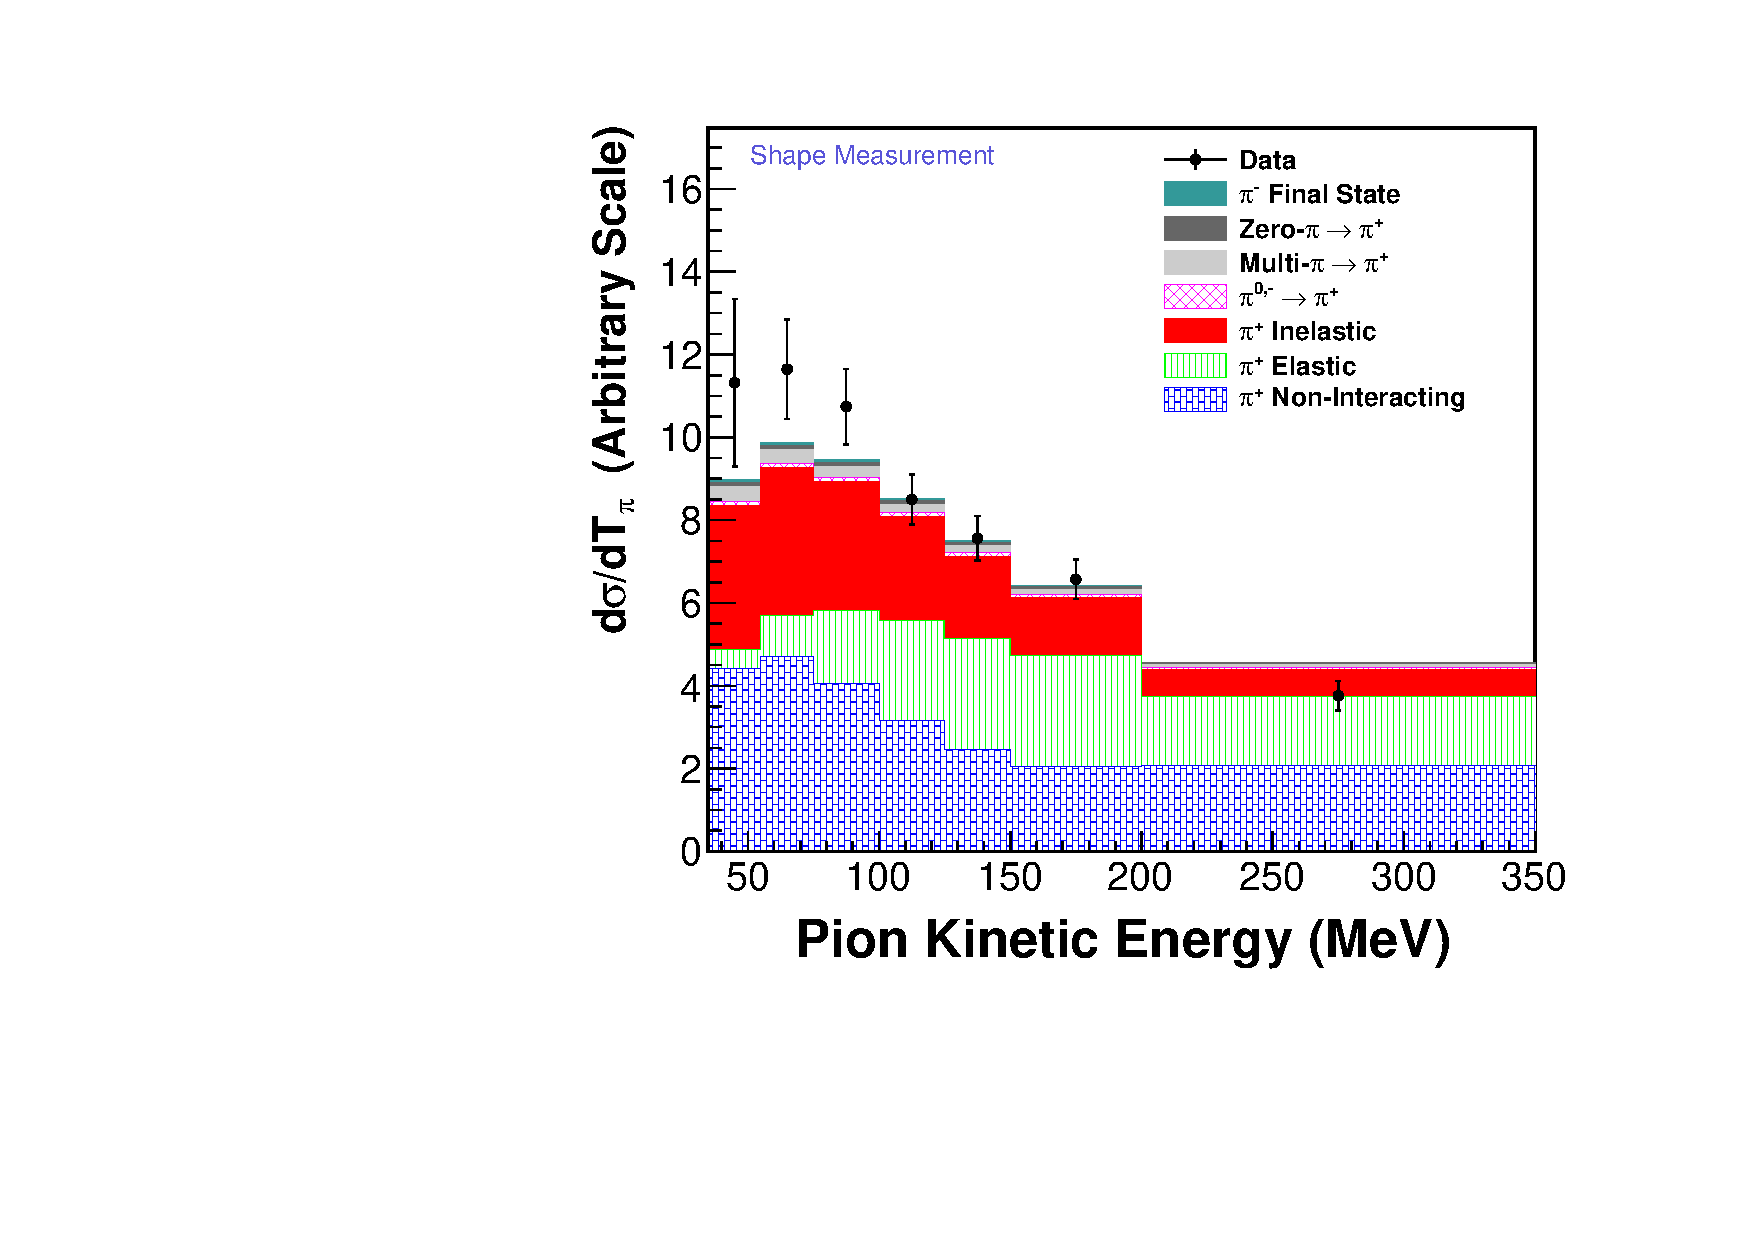
\includegraphics[width=\columnwidth]{figures/crossSection_fsiSummary_pi_ke_an} % shrink to fit PL 
%\vspace{-7pt}
\caption{The measured shape of $d\sigma / dT_\pi$ and a breakdown of the GENIE calculation
by FSI channel.  Coherent pion production and hydrogen interactions are included in the ``Non-Interacting'' category.  
The simulation is normalized to the integral of the data.}
    %\vspace{-10pt}
\label{fig:pike-1pi-AN-FSI}
\end{figure}
 
\begin{figure}[!htp]
\centering
  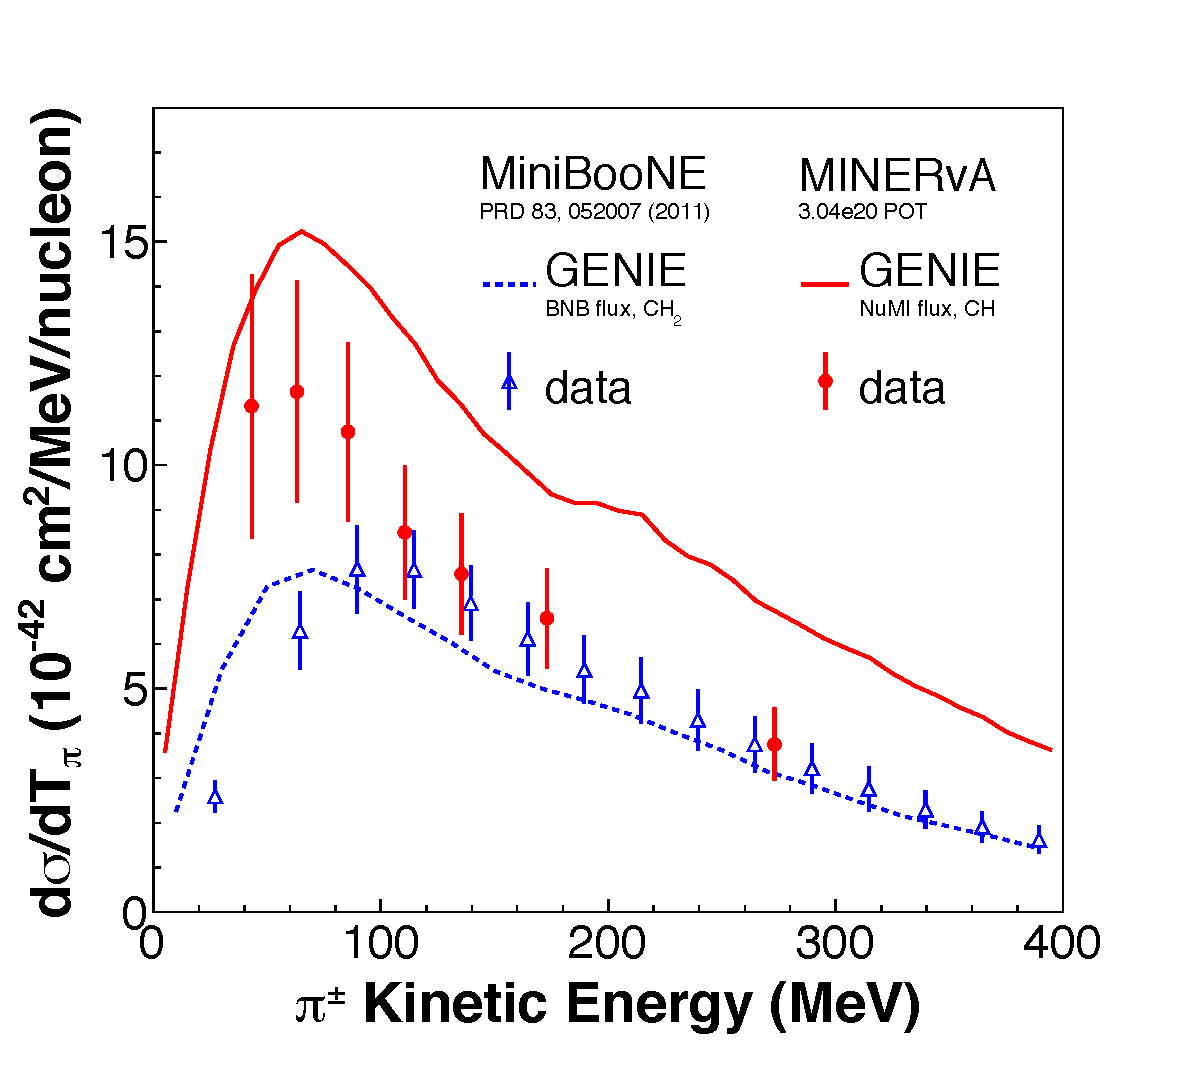
\includegraphics[width=0.9\columnwidth]{figures/mboone_comp}
    %\vspace{-7pt}
\caption{Comparison between the \minerva and \miniboone~\cite{miniboone_piprod} $d\sigma/d T_\pi$ data via the corresponding GENIE 2.6.2 ``hA FSI'' predictions.
Error bars indicate the total uncertainty.}
    %\vspace{-10pt}
\label{fig:mb-comp}
\end{figure} 
 
Since these data favor different calculations than the \miniboone 
data~\cite{Rodrigues:2014jfa}, a comparison of the two data sets is interesting.
Figure~\ref{fig:mb-comp} compares this measurement of \cconepi $d\sigma/dT_\pi$ with that 
of \miniboone along with the two corresponding GENIE predictions for 
the appropriate neutrino fluxes~\cite{miniboone_flux} and signal definitions.  
\minerva measures higher energy and higher 
$Q^2$ neutrino interactions than does \miniboone, but the $W$ and 
$T_\pi$ kinematic ranges overlap significantly.  \minerva reports
the cross section at $W<$ 1.4 GeV while \miniboone 
selects events with reconstructed $W<$ 1.35 GeV and uses the NUANCE event generator~\cite{NUANCE} 
to measure the cross section over the full $W$ range; 
GENIE predicts that 24\% of the \miniboone cross section result is at 
$W>$ 1.4 GeV. All these considerations lead to differences in the 
contributions due to $\Delta$ excitation and non-resonant 
backgrounds, but the key feature of attenuation due to pion FSI 
is expected to be similar. 

The \minerva and \miniboone results have a similar shape and magnitude above 
$T_\pi=100$~MeV in Fig.~\ref{fig:mb-comp}.  The shape agreement indicates some 
consistency in the pion absorption FSI process, while the agreement in 
magnitude is unexpected when considering the different $E_{\nu}$ and $W$ ranges 
of the measurements and is not presently described by any models.  
In fact, the \minerva cross section at higher \Tpi would nominally be
larger than the \miniboone result 
because the cross section for pion production
from nucleon targets rises with increasing $E_\nu$.
The shape disagreement below 100~MeV is also not explained 
by current models.  The GENIE model predicts the 
shape but overpredicts the level of the \minerva data (see Fig.~\ref{fig:pike-1pi} for shape), while it 
predicts the magnitude but not the shape of the MiniBooNE 
data.  
The same trend is seen with the GiBUU calculation, as shown in 
Ref.~\cite{gibuu-pi}.  

\begin{figure}[ht]
\centering
\subfloat[] {
    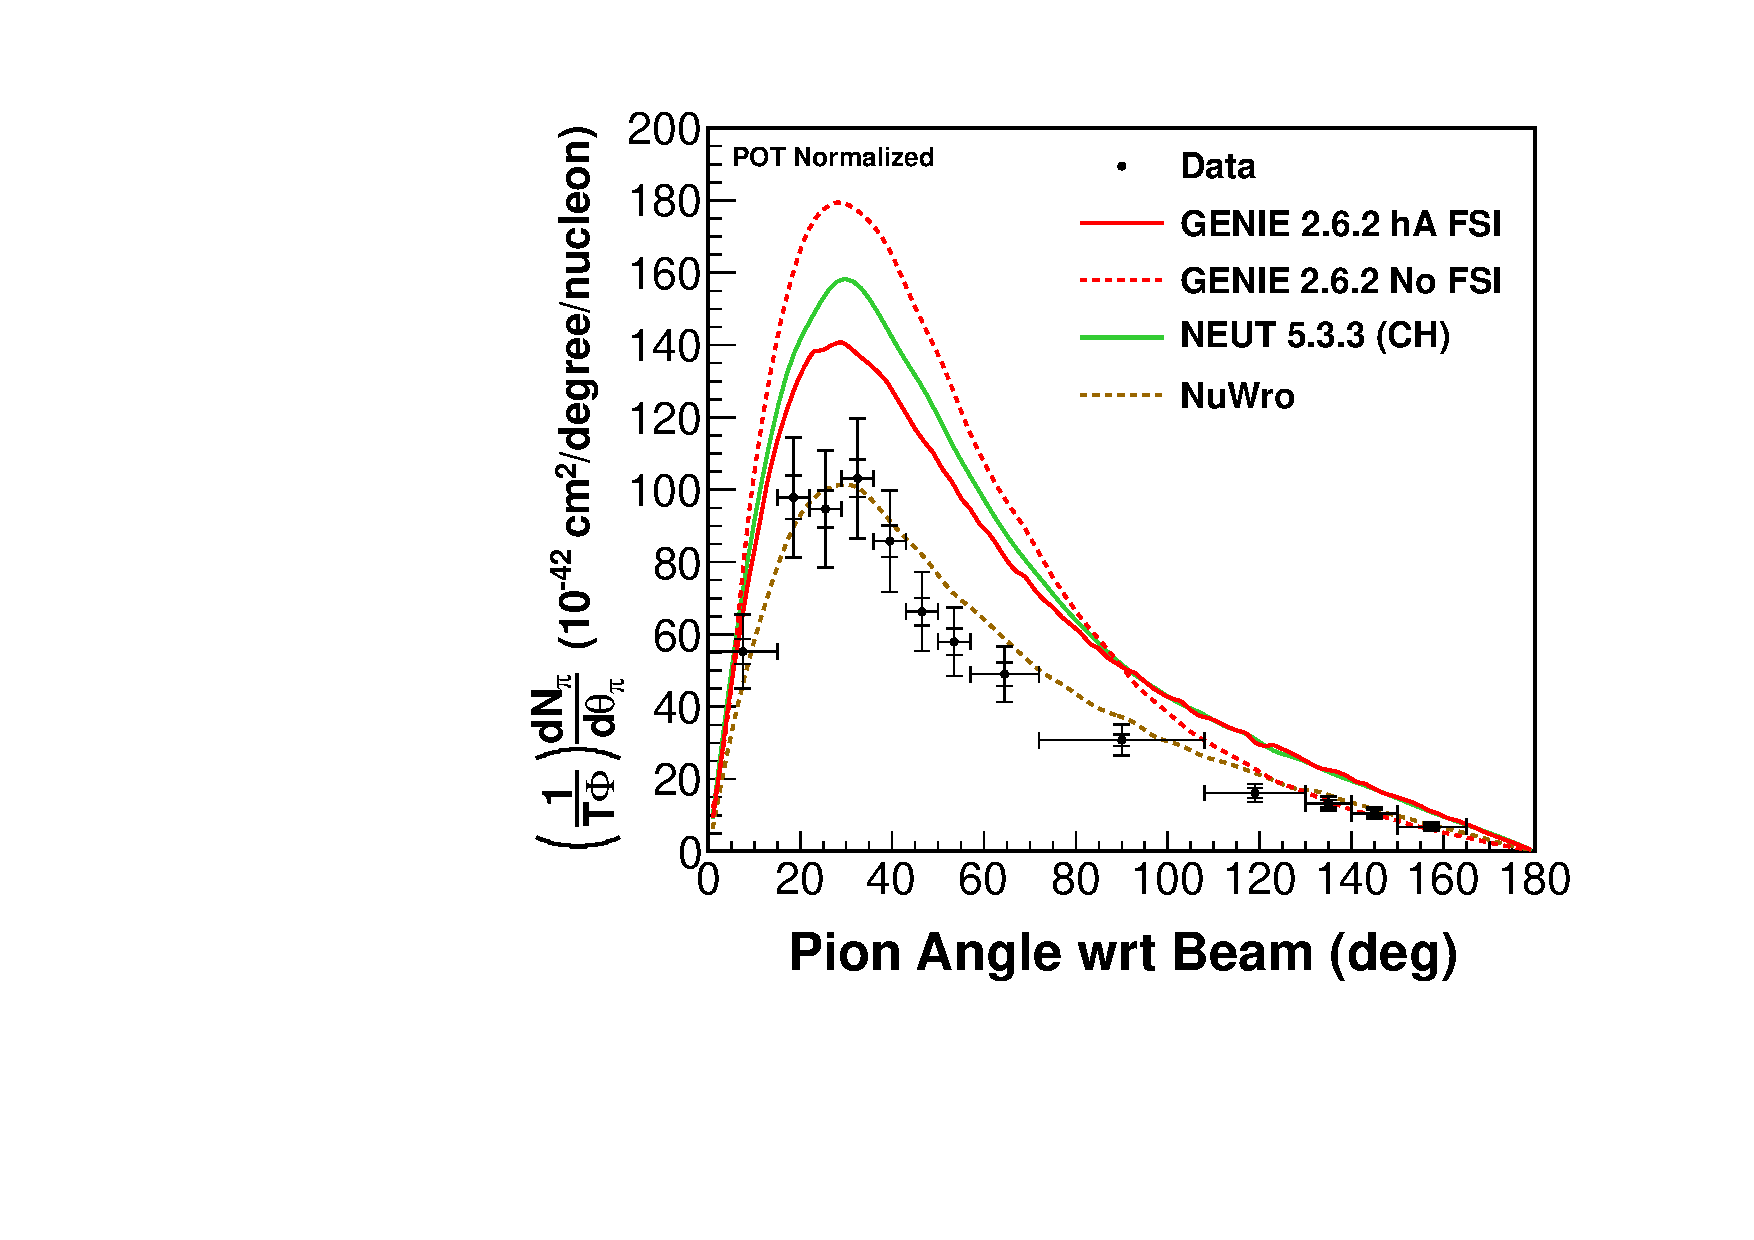
\includegraphics[width=\columnwidth]{figures/modelComp_POT_pi_theta_Npi}
}
\qquad
\subfloat[] {
    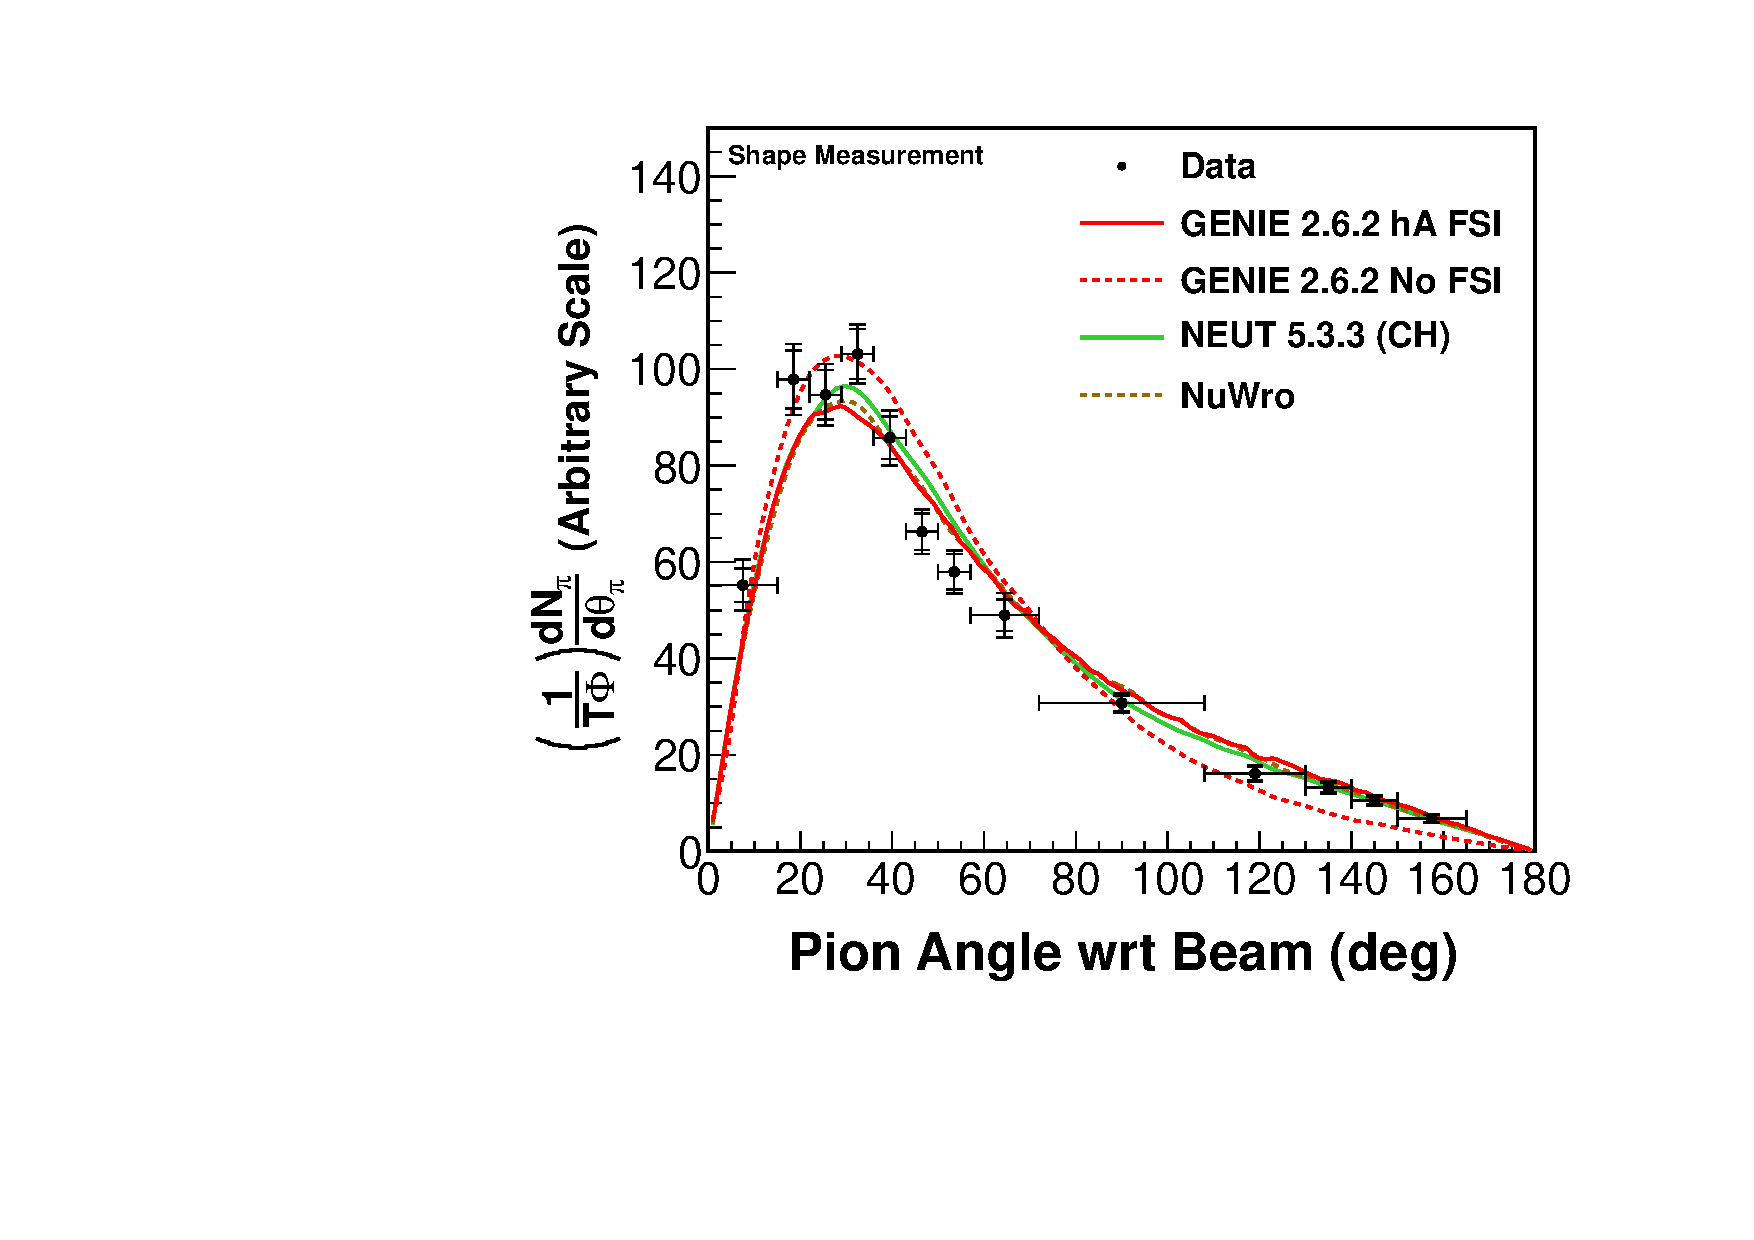
\includegraphics[width=\columnwidth]{figures/modelComp_AN_pi_theta_Npi}
}
%    \vspace{-7pt}
\caption{\ccpi $(1/T\Phi)(dN_{\pi} / d\theta_\pi)$ (top) and its shape (bottom) compared to the GENIE, NEUT, and NuWro models.
The inner (outer) error bars correspond to the statistical (total) uncertainties.}
%    \vspace{-10pt}
\label{fig:piangle-Npi-POT}
\end{figure}

\begin{figure}[ht]
\centering
\subfloat[] {
    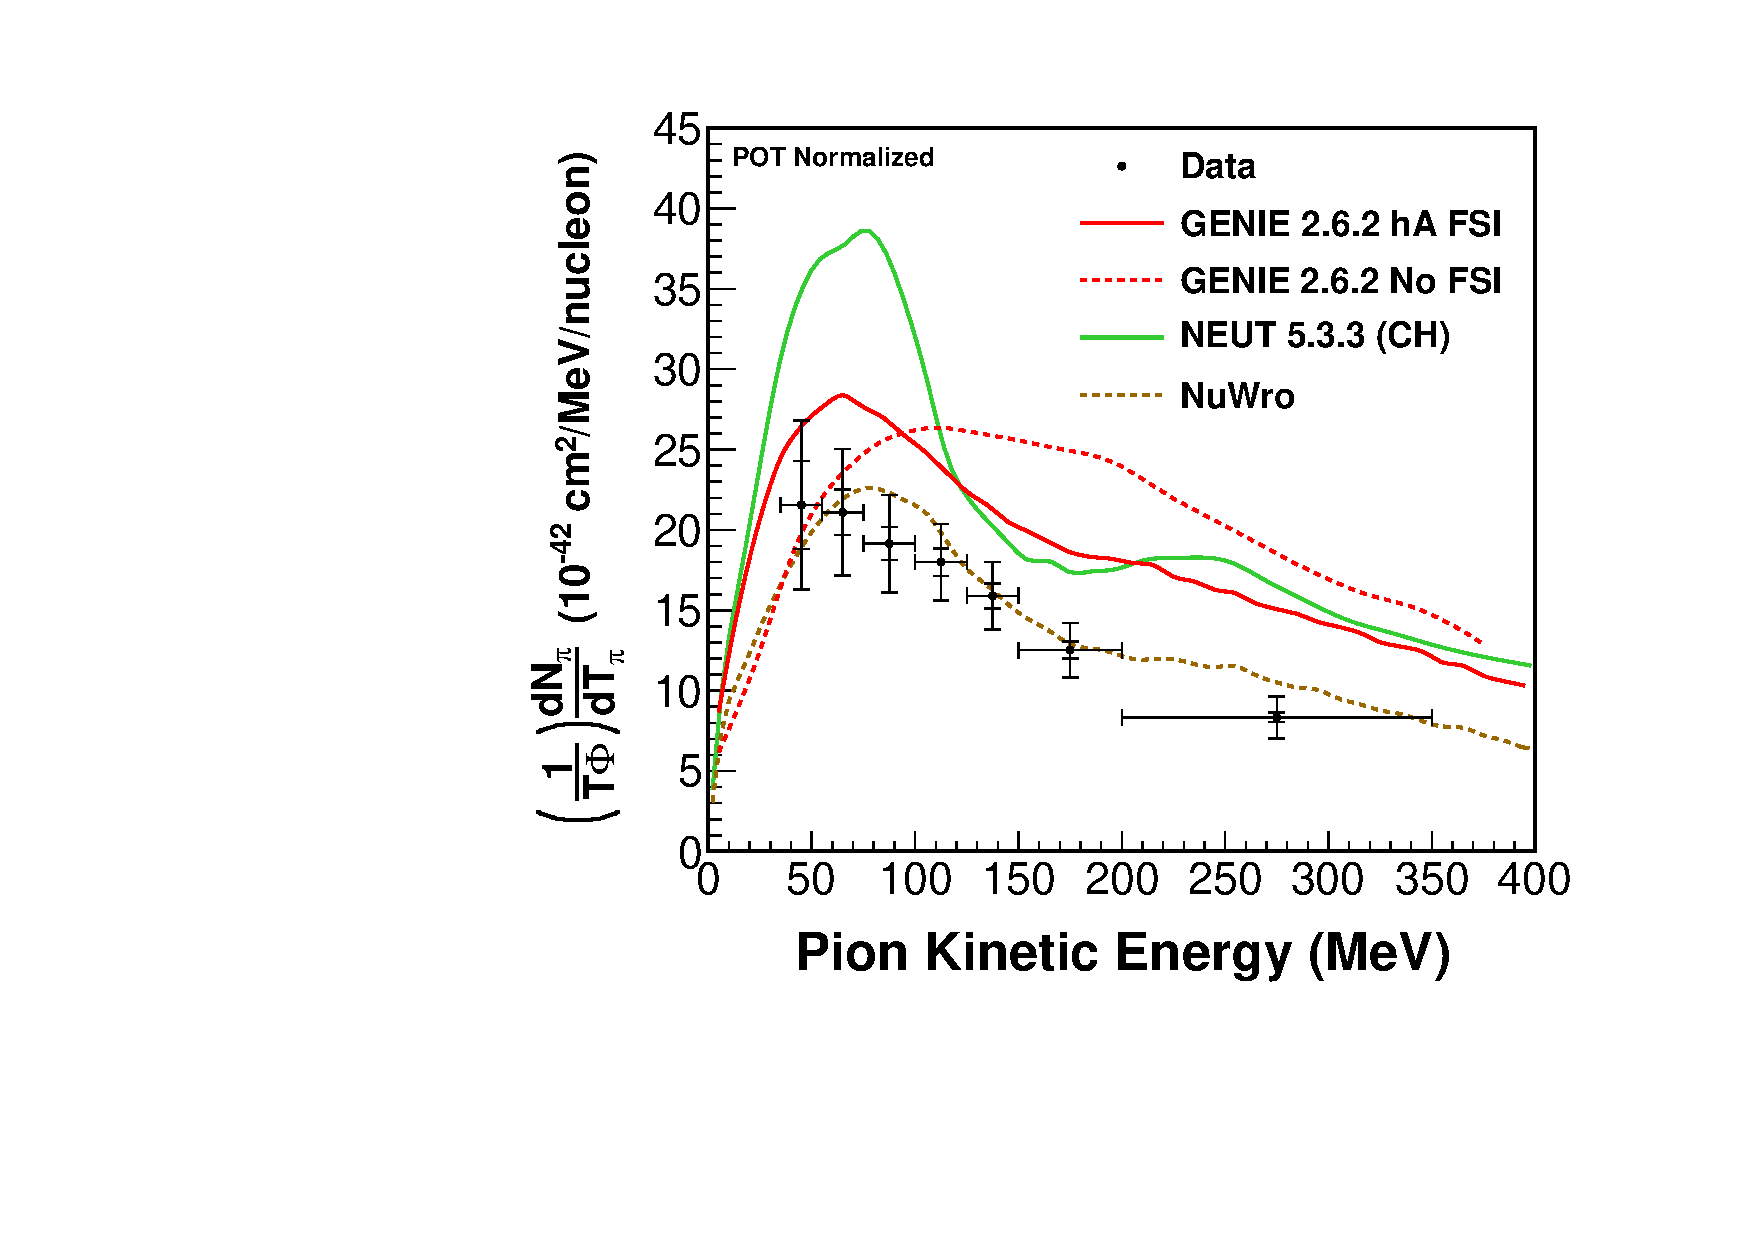
\includegraphics[width=\columnwidth]{figures/modelComp_POT_pi_ke_Npi}
}
\qquad
\subfloat[] {
    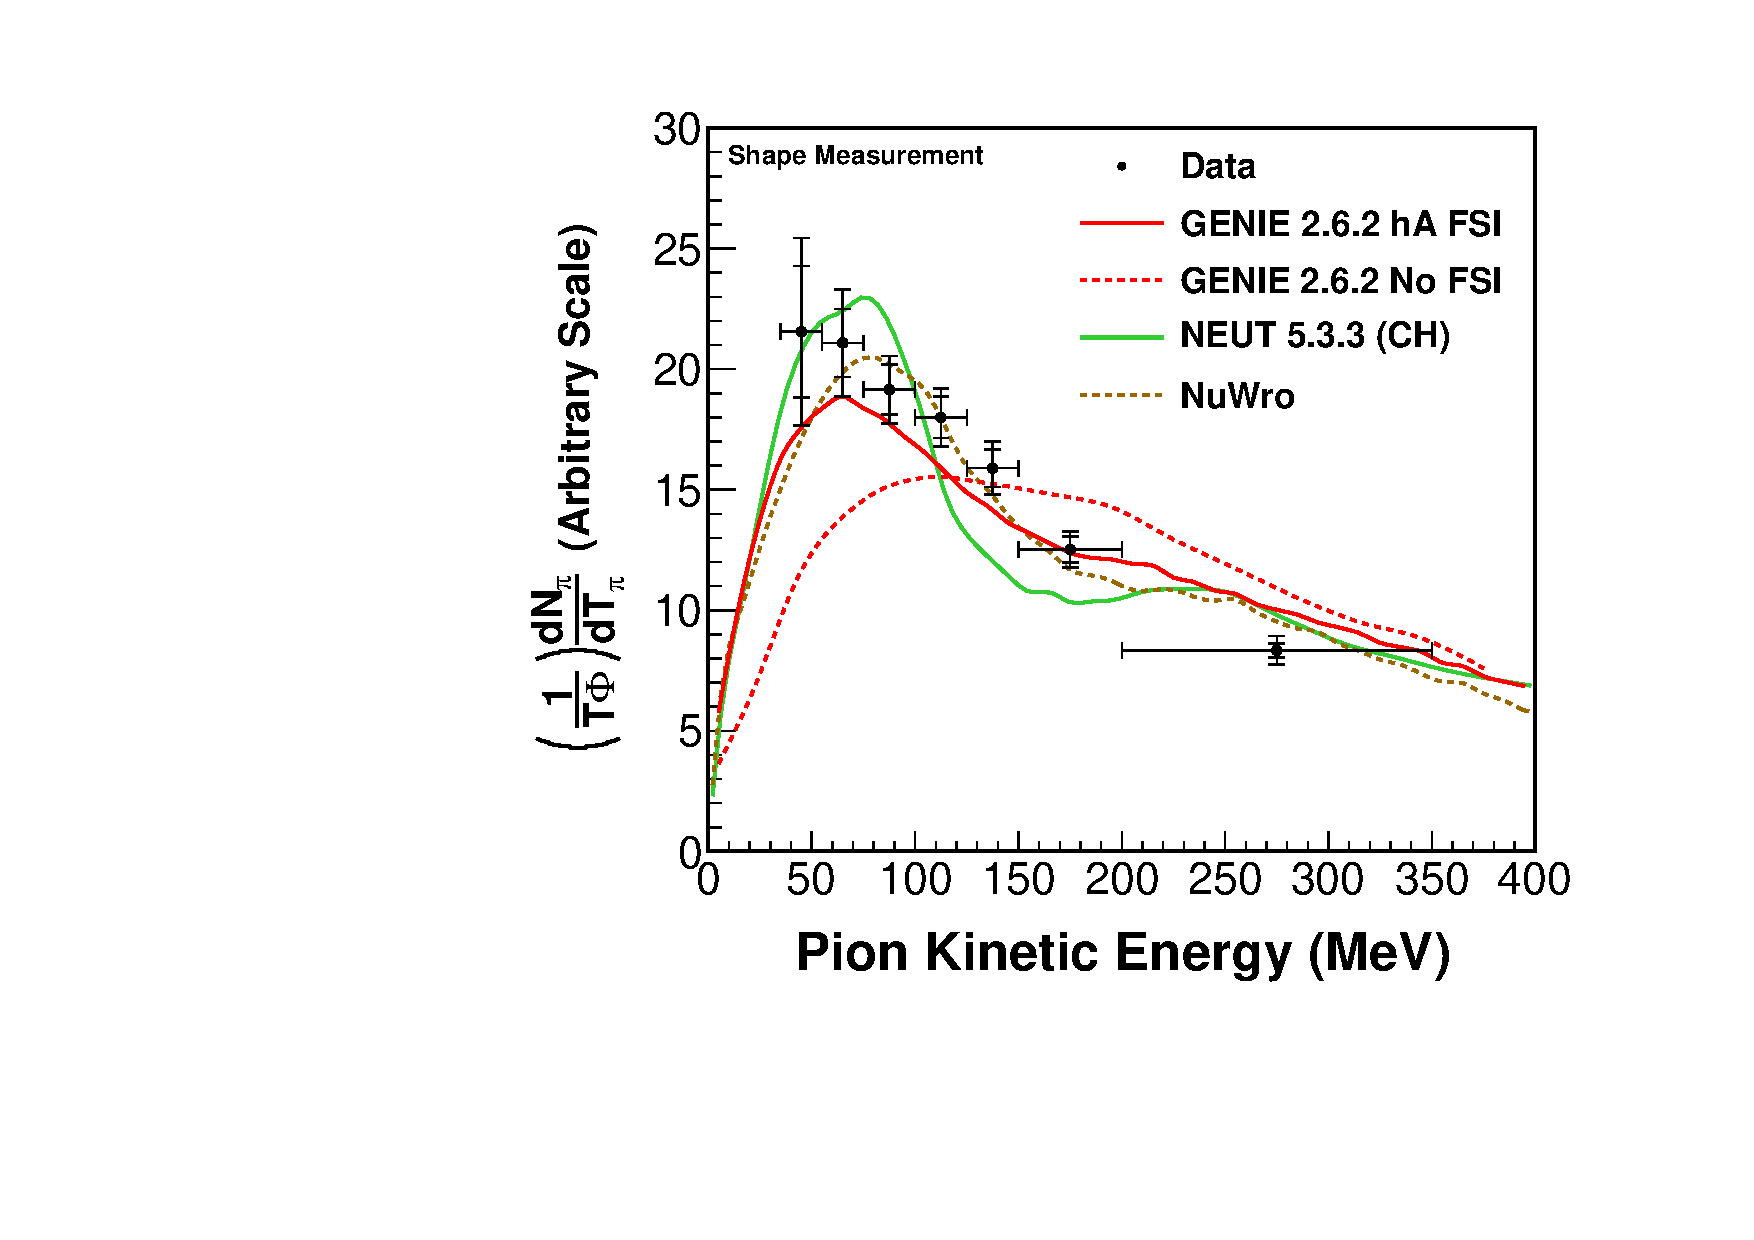
\includegraphics[width=\columnwidth]{figures/modelComp_AN_pi_ke_Npi}
}
%    \vspace{-7pt}
\caption{\ccpi $(1/T\Phi)(dN_{\pi} / dT_\pi)$ (top) and its shape (bottom) compared to the GENIE, NEUT, and NuWro models.
The inner (outer) error bars correspond to the statistical (total) uncertainties.}
%    \vspace{-10pt}
\label{fig:pike-Npi-POT}
\end{figure}

\subsection{\ccpi\ results}
Extension of the maximum $W$ from 1.4 to 1.8 GeV in the \ccpi
analysis includes additional nonresonant processes and $N^*$ resonances at high mass. For each event, 
more than one charged pion can be counted 
(see Section~\ref{sec:xs}), which causes these distributions to be sensitive to pion-producing FSI processes 
in higher-multiplicity events.  GENIE predicts that 19\% of the \ccpi charged pions come from two-pion events, and 
5\% come from events with three or more charged pions.

Figures~\ref{fig:piangle-Npi-POT} and~\ref{fig:pike-Npi-POT} show 
the results
of the \ccpi analysis as well as the GENIE (no FSI and with FSI),
NEUT, and NuWro predictions.  The data distributions are very
similar in shape to Figures~\ref{fig:piangle-1pi} and~\ref{fig:pike-1pi}
even though the total cross section is roughly 50\% larger, and the relative 
normalization of the GENIE prediction to the data does not change.  The NuWro 
prediction for the total \ccpi cross section improves slightly relative to its 
prediction for the \cconepi channel, while NEUT predicts a much larger increase 
in final state pions, particularly at \Tpi $<$ 100 MeV,  for the higher $W$ processes.  

\section{Summary}
\label{sec:summary}
This paper presents measurements of neutrino-induced pion production from 
a CH target and compares them to models with different FSI treatments and 
to the \miniboone measurement of the same process.  These data provide 
new information about the neutrino energy dependence of resonant pion production 
and can be used to place strong constraints on FSI. More generally, 
they provide an observational foundation for improving both the 
background and signal predictions needed for precise oscillation parameter 
measurements. 

Both the $d\sigma/d\theta_\pi$ and $d\sigma/dT_\pi$ distribution
shapes strongly favor models with FSI implemented as a full or effective cascade algorithm. 
For the \cconepi 
analysis, the calculations with FSI, NEUT and NuWro are in good 
agreement with the data while GENIE predicts cross sections
that are too large.  The distribution shape contains the most information
about FSI.  At $T_\pi$ greater than 100~MeV, 
where pion FSI effects largely deplete the yield, 
\minerva and \miniboone have similar shape.  However, the similarity
in magnitude is not expected.  There are also 
significant normalization and shape discrepancies between the two 
measurements below 100~MeV in comparison with the GENIE calculation.
A decomposition of the FSI channels in the GENIE calculation suggest 
that an increased inelastic contribution may improve agreement with the data.

For the \ccpi analysis, data results are similar to the \cconepi analysis.
However, differences among the models employed in the generators
produce significant changes with respect to the data.
The shape is strongly affected by FSI and the magnitude
disagreement can come from problems within the Monte Carlo models.

It is clear that the underlying pion production models and perhaps
other parts of the neutrino interaction will have to be 
modified to reproduce both data sets, which will in turn help improve 
predictions for oscillation experiments.


